\documentclass{article}
\usepackage{fullpage}
\usepackage{amsmath,amsthm,amsrefs,amssymb}
%\usepackage[utf8x]{inputenc}
\usepackage{hyperref}
\newtheorem{lemma}{Lemma}
\newtheorem{theorem}{Theorem}
\newtheorem{corollary}{Corollary}
\newtheorem{proposition}{Proposition}
\newtheorem{conjecture}{Conjecture}
\newtheorem{wellknown}{Standard Knowledge}
\newtheorem{problem}[conjecture]{Problem}
\theoremstyle{definition}
\newtheorem{definition}{Definition}
\newtheorem{sdef}{Standard Term}

\newcommand{\N}{\mathbb{N}}
\newcommand{\NZ}{\N_0}
\glossary{$\NZ$: natural numbers including 0}
\newcommand{\Z}{\mathbb{Z}}
\newcommand{\Q}{\mathbb{Q}}
\newcommand{\QP}{\mathbb{Q}_+}
\newcommand{\R}{\mathbb{R}}
\newcommand{\C}{\mathbb{C}}
\newcommand{\RP}{\mathbb{R}_+}
\newcommand{\RI}{\R_{>1}}
\newcommand{\RII}{\R_{\ge 1}}
\newcommand{\then}{\Longrightarrow}
\newcommand{\wo}{\setminus}
\newcommand{\propref}[1]{proposition \ref{#1}}
\newcommand{\defref}[1]{definition \ref{#1}}
\newcommand{\rh}{\varrho}
\newcommand{\eps}{\varepsilon}
\newcommand{\ph}{\varphi}
\newcommand{\sexp}{\operatorname{sexp}}
\newcommand{\slog}{\operatorname{slog}}
\newcommand{\spow}{\operatorname{spow}}
\newcommand{\rsexp}{\sexp^{\mathfrak{R}}}
\newcommand{\rslog}{\slog^{\mathfrak{R}}}
\newcommand{\rusexp}{\sexp^{\mathfrak{R}^+}}
\newcommand{\ruslog}{\slog^{\mathfrak{R}^+}}
\newcommand{\msexp}{\sexp^{\mathfrak{M}}}
\newcommand{\mslog}{\slog^{\mathfrak{M}}}
\newcommand{\ksexp}{\sexp^{\mathfrak{C}}}
\newcommand{\kslog}{\slog^{\mathfrak{C}}}
\newcommand{\isexp}{\sexp^{\mathfrak{I}}}
\newcommand{\islog}{\slog^{\mathfrak{I}}}

\newcommand{\mt}[1]{\quad\mbox{#1}\quad}
\newcommand{\abs}[1]{\left|#1\right|}
\newcommand{\I}{\mathrm{i}}
\newcommand{\di}{\mathrm{d}} %*d*elta of *i*ntegration

%commands by Kouznetsov begin
\usepackage{graphics}
\usepackage{rotating}
\newcommand \sx {\scalebox}
\newcommand \rme {\mathrm{e}}
\newcommand \rot {\begin{rotate}}
\newcommand \ero {\end{rotate}}
\newcommand \rf[1] {(\ref{#1})}
\newcommand \iL[1] {~ \label{#1} ~~~[#1]}
\newcommand \ing {\includegraphics}
\newcommand \rmi {\mathrm{i}}
\newcommand \be {\begin{eqnarray}}
\newcommand \ee {\end{eqnarray}}
\newcommand \eL[1] {\iL{#1} \end{eqnarray}}
%commands by Kouznetsov end

\DeclareMathOperator{\id}{id} %locally with \operatorname{id}

% Local Variables:
% TeX-master: "main"
% End:


\newcommand{\tet}{\operatorname{[4]}}
\begin{document}

%\input{dec}
\Large
In this section, the holomorphic solutions $F$ of equation
\be
F(z\!+\!1)= \exp\!\left(\frac{F(z)}{\rme}\right)
\eL{e1ee}
are considered.
%\end{document}

At the traditional approach, the iterational procedure for the approximation of the soution 
converges slwly if at all.

TODO: Henryk, please, copypast here your explanation why the traditional approach fails.

DODO: Dmitrii plans to type there the descriprion of figures.

As usually, we specify the superexponential, indicating the value at zero as subscript.
we consider the two superexponentials, $F=F_1$ and $F=F_3$ such that
\be
F_1(0)=1 ~~,~~~~d_3(0)=3~~;
\eL{e1e13}
as in the case of $b=2$, we choose the smallest integer among the range of values of the 
growing superexponential along the real axis, as value at zero.
Behavior of these two superexponentials along the real axix is shown in 
%\end{document}
figure \ref{fig1e1fre}.

\begin{figure}
\begin{center}
{\normalsize
\sx{1.2}{\begin{picture}(320,220)
\put(0,0){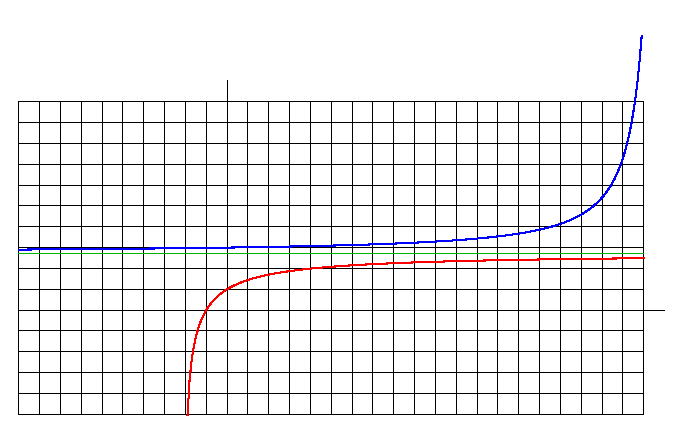
\includegraphics{e1e/fige1efre}}
%\put(220,14){\sx{.7}{$\ln b$}}
\put( 95,157){\sx{1.}{$y$}}
\put( 95,129){\sx{1.}{$8$}}
\put( 95,109){\sx{1.}{$6$}}
\put( 95, 89){\sx{1.}{$4$}}
\put( 95, 69){\sx{1.}{$2$}}
\put( 88, 28){\sx{1.}{$-2$}}
\put( 88,  8){\sx{1.}{$-4$}}
\put(-11, 43){\sx{1.}{$-\!10$}}
\put( 12, 43){\sx{1.}{$-8$}}
\put( 32, 43){\sx{1.}{$-6$}}
\put( 52, 43){\sx{1.}{$-4$}}
\put( 72, 43){\sx{1.}{$-2$}}
\put(119, 43){\sx{1.}{$2$}}
\put(139, 43){\sx{1.}{$4$}}
\put(159, 43){\sx{1.}{$6$}}
\put(179, 43){\sx{1.}{$8$}}
\put(195, 43){\sx{1.}{$10$}}
\put(216, 43){\sx{1.}{$12$}}
\put(236, 43){\sx{1.}{$14$}}
\put(256, 43){\sx{1.}{$16$}}
\put(276, 43){\sx{1.}{$18$}}
\put(304, 44){\sx{1.}{$x$}}
\put(302,170){\sx{1.}{$y\!=\!\mathrm{F}_{3}(x)$}}
\put(304, 80){\sx{1.}{$y\!=\!\rme$}}
\put(304, 70){\sx{1.}{$y\!=\!\mathrm{F}_{1}(x)$}}
\end{picture}}
}
\end{center}
\caption{Tho superexponentials to base $~b\!=\!\exp(1/\rme)~$ versus real argument
by equations e1e1 and e1e3;
the horizontal line shows the asymptotic $~y\!=\!\rme~$.
%
\iL{fig1e1fre}
}
\end{figure}
%\end{document}

The algorithm of evaluation described below does not imply 
that the argument of the superexponential is real; so, in figure 
\ref{fige1e}
, functions $F_{1}$ and $F_{3}$ and their inverse functions 
$G_{1}=F_{1}^{-1}$ and $G_{3}=F_{3}^{-1}$ are shown in the complex plane.

\begin{figure}
\begin{center}
\normalsize{
\sx{.72}{\begin{picture}(220,220)
\put(0,0){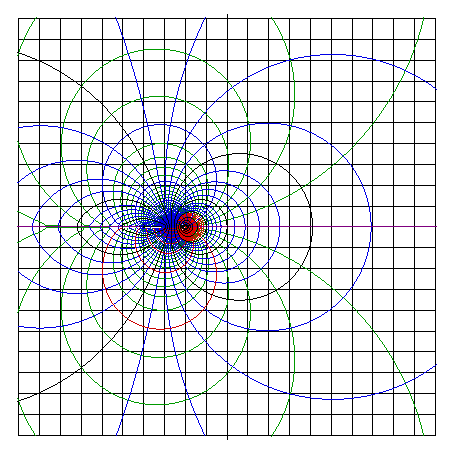
\includegraphics{e1e/fige1etf}}
\put(-11,204){\sx{1}{$\Im(z)$}}
\put( -5,179){\sx{1}{$8$}}
\put( -5,159){\sx{1}{$6$}}
\put( -5,139){\sx{1}{$4$}}
\put( -5,119){\sx{1}{$2$}}
\put( -5, 99){\sx{1}{$0$}}
\put(-13, 79){\sx{1}{$-2$}}
\put(-13, 59){\sx{1}{$-4$}}
\put(-13, 39){\sx{1}{$-6$}}
\put(-13, 19){\sx{1}{$-8$}}
%\put(-13, 79){\sx{1}{$-6$}}
\put(192,-7){\sx{1}{$\Re(z)$}}
\put(179,-6){\sx{.9}{$8$}}
\put(159,-6){\sx{.9}{$6$}}
\put(139,-6){\sx{.9}{$4$}}
\put(119,-6){\sx{.9}{$2$}}
\put( 99,-6){\sx{.9}{$0$}}
\put( 73,-6){\sx{.9}{$-2$}}
\put( 53,-6){\sx{.9}{$-4$}}
\put( 33,-6){\sx{.9}{$-6$}}
\put( 13,-6){\sx{.9}{$-8$}}
%\put(220,14){\sx{.7}{$\ln b$}}
\end{picture}}
\sx{.72}{\begin{picture}(220,220)
\put(0,0){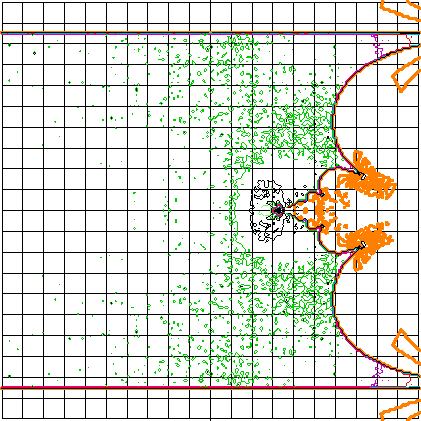
\includegraphics{e1e/fige1etfi}}
\put(-11,204){\sx{1}{$\Im(z)$}}
\put( -5,179){\sx{1}{$8$}}
\put( -5,159){\sx{1}{$6$}}
\put( -5,139){\sx{1}{$4$}}
\put( -5,119){\sx{1}{$2$}}
\put( -5, 99){\sx{1}{$0$}}
\put(-13, 79){\sx{1}{$-2$}}
\put(-13, 59){\sx{1}{$-4$}}
\put(-13, 39){\sx{1}{$-6$}}
\put(-13, 19){\sx{1}{$-8$}}
%\put(-13, 79){\sx{1}{$-6$}}
\put(192,-7){\sx{1}{$\Re(z)$}}
\put(179,-6){\sx{.9}{$8$}}
\put(159,-6){\sx{.9}{$6$}}
\put(139,-6){\sx{.9}{$4$}}
\put(119,-6){\sx{.9}{$2$}}
\put( 99,-6){\sx{.9}{$0$}}
\put( 73,-6){\sx{.9}{$-2$}}
\put( 53,-6){\sx{.9}{$-4$}}
\put( 33,-6){\sx{.9}{$-6$}}
\put( 13,-6){\sx{.9}{$-8$}}
%\put(220,14){\sx{.7}{$\ln b$}}
\end{picture}}
\sx{.72}{\begin{picture}(200,220)
\put(0,0){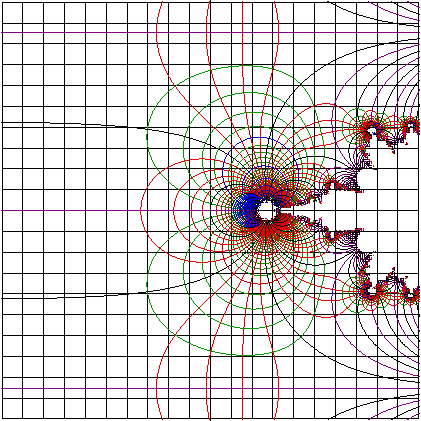
\includegraphics{e1e/fige1eti}}
\put(-11,204){\sx{1}{$\Im(z)$}}
\put( -5,179){\sx{1}{$8$}}
\put( -5,159){\sx{1}{$6$}}
\put( -5,139){\sx{1}{$4$}}
\put( -5,119){\sx{1}{$2$}}
\put( -5, 99){\sx{1}{$0$}}
\put(-13, 79){\sx{1}{$-2$}}
\put(-13, 59){\sx{1}{$-4$}}
\put(-13, 39){\sx{1}{$-6$}}
\put(-13, 19){\sx{1}{$-8$}}
\put(192,-7){\sx{1}{$\Re(z)$}}
\put(179,-6){\sx{.9}{$8$}}
\put(159,-6){\sx{.9}{$6$}}
\put(139,-6){\sx{.9}{$4$}}
\put(119,-6){\sx{.9}{$2$}}
\put( 99,-6){\sx{.9}{$0$}}
\put( 73,-6){\sx{.9}{$-2$}}
\put( 53,-6){\sx{.9}{$-4$}}
\put( 33,-6){\sx{.9}{$-6$}}
\put( 13,-6){\sx{.9}{$-8$}}
\end{picture}}
\vskip 6mm

\sx{.72}{\begin{picture}(220,220)
\put(0,0){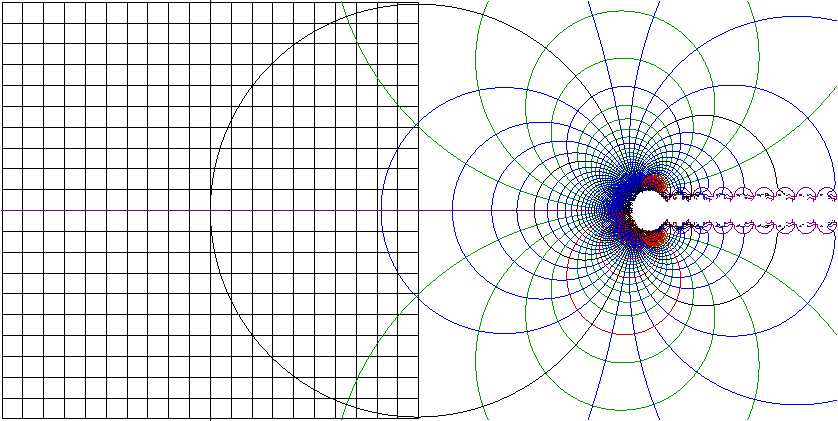
\includegraphics{e1e/fige1egf}}
\put(-11,204){\sx{1}{$\Im(z)$}}
\put( -5,179){\sx{1}{$8$}}
\put( -5,159){\sx{1}{$6$}}
\put( -5,139){\sx{1}{$4$}}
\put( -5,119){\sx{1}{$2$}}
\put( -5, 99){\sx{1}{$0$}}
\put(-13, 79){\sx{1}{$-2$}}
\put(-13, 59){\sx{1}{$-4$}}
\put(-13, 39){\sx{1}{$-6$}}
\put(-13, 19){\sx{1}{$-8$}}
\put(192,-7){\sx{1}{$\Re(z)$}}
\put(179,-6){\sx{.9}{$8$}}
\put(159,-6){\sx{.9}{$6$}}
\put(139,-6){\sx{.9}{$4$}}
\put(119,-6){\sx{.9}{$2$}}
\put( 99,-6){\sx{.9}{$0$}}
\put( 73,-6){\sx{.9}{$-2$}}
\put( 53,-6){\sx{.9}{$-4$}}
\put( 33,-6){\sx{.9}{$-6$}}
\put( 13,-6){\sx{.9}{$-8$}}
\end{picture}}
\sx{.72}{\begin{picture}(220,220)
%\put(0,0){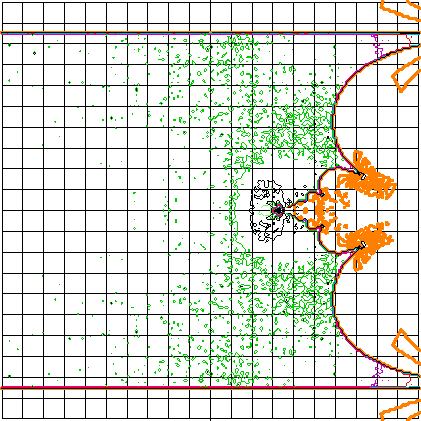
\includegraphics{e1e/fige1etfi}}
\end{picture}}
\sx{.72}{\begin{picture}(200,220)
\put(0,0){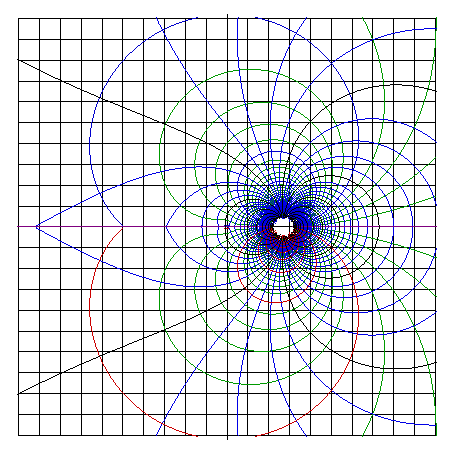
\includegraphics{e1e/fige1egi}}
\put(-11,204){\sx{1}{$\Im(z)$}}
\put( -5,179){\sx{1}{$8$}}
\put( -5,159){\sx{1}{$6$}}
\put( -5,139){\sx{1}{$4$}}
\put( -5,119){\sx{1}{$2$}}
\put( -5, 99){\sx{1}{$0$}}
\put(-13, 79){\sx{1}{$-2$}}
\put(-13, 59){\sx{1}{$-4$}}
\put(-13, 39){\sx{1}{$-6$}}
\put(-13, 19){\sx{1}{$-8$}}
\put(192,-7){\sx{1}{$\Re(z)$}}
\put(179,-6){\sx{.9}{$8$}}
\put(159,-6){\sx{.9}{$6$}}
\put(139,-6){\sx{.9}{$4$}}
\put(119,-6){\sx{.9}{$2$}}
\put( 99,-6){\sx{.9}{$0$}}
\put( 73,-6){\sx{.9}{$-2$}}
\put( 53,-6){\sx{.9}{$-4$}}
\put( 33,-6){\sx{.9}{$-6$}}
\put( 13,-6){\sx{.9}{$-8$}}
\end{picture}}
}\end{center}
\caption{
Superexponentials to base $\exp(1/\rme)$ and their inverse functions:
$F_1(z)$, left, top; 
$F_1^{-1}(z)$, right, top; residual $D_{\rme}$, top, center;
$F_3(z)$, left, bottom; 
$F_3^{-1}(z)$, right, bottom.
\iL{fige1e}
}
\end{figure}


\end{document}
